\documentclass[11pt]{article}
\usepackage{amsmath,amssymb,amsthm}
\usepackage{graphicx}
\usepackage{url}
\usepackage{hyperref}
\usepackage{color}
\usepackage{algorithm,algorithmic}
\usepackage[T1]{fontenc}

\hypersetup{
    colorlinks=true,
    linkcolor=blue,
    filecolor=magenta,      
    urlcolor=cyan,
}


\newcommand{\INPUT}{\item[{\bf Input:}]}
\newcommand{\OUTPUT}{\item[{\bf Output:}]}
\newcommand{\RR}{{\mathbb R}}
\newcommand{\myvec}[1]{\mathbf{#1}}
\newcommand{\ignore}[1]{}%


\DeclareMathOperator*{\E}{\mathbb{E}}
\let\Pr\relax
\DeclareMathOperator*{\Pr}{\mathbb{P}}
%\DeclareMathOperator*{\myv}{\mathbf{#1}}
\newcommand{\mv}[1]{\mathbf{#1}}
\newcommand{\mynorm}[1]{\|{#1}\|}


\newcommand{\eps}{\varepsilon}
\newcommand{\inprod}[1]{\left\langle #1 \right\rangle}

\newcommand{\handout}[5]{
  \noindent
  \begin{center}
  \framebox{
    \vbox{
      %\hbox to 5.78in { {\bf AM 221: Advanced Optimization } \hfill #2 }
            \hbox to 6.38in { {\bf AM 221: Advanced Optimization } \hfill #2 }
      \vspace{4mm}
      %\hbox to 5.78in { {\Large \hfill #5  \hfill} }
            \hbox to 6.38in { {\Large \hfill #5  \hfill} }
      \vspace{2mm}
            \hbox to 6.38in { {\em #3 \hfill #4} }
      %\hbox to 5.78in { {\em #3 \hfill #4} }
    }
  }
  \end{center}
  \vspace*{4mm}
}

\newcommand{\lecture}[3]{\handout{#1}{#2}{#3}{Lecture #1}}
\newcommand{\homework}[3]{\handout{#1}{#2}{#3}{Problem Set #1}}
\newcommand{\sect}[3]{\handout{#1}{#2}{#3}{Section #1}}

\newtheorem{theorem}{Theorem}
\newtheorem{corollary}[theorem]{Corollary}
\newtheorem{lemma}[theorem]{Lemma}
\newtheorem{observation}[theorem]{Observation}
\newtheorem{proposition}[theorem]{Proposition}
\newtheorem{definition}[theorem]{Definition}
\newtheorem{claim}[theorem]{Claim}
\newtheorem{fact}[theorem]{Fact}
\newtheorem{assumption}[theorem]{Assumption}

\newtheorem*{theorem*}{Theorem}
\newtheorem*{corollary*}{Corollary}
\newtheorem*{conjecture*}{Conjecture}
\newtheorem*{lemma*}{Lemma}
\newtheorem*{thm*}{Theorem}
\newtheorem*{prop*}{Proposition}
\newtheorem*{obs*}{Observation}
\newtheorem*{definition*}{Definition}
\theoremstyle{remark}
\newtheorem{remark}[theorem]{Remark}
\newtheorem*{example}{Example}
\newtheorem*{rem*}{Remark}
\newtheorem*{rec*}{Recommendation}


% 1-inch margins, from fullpage.sty by H.Partl, Version 2, Dec. 15, 1988.
\topmargin 0pt
\advance \topmargin by -\headheight
\advance \topmargin by -\headsep
\textheight 8.9in
\oddsidemargin 0pt
\evensidemargin \oddsidemargin
\marginparwidth 0.5in
\textwidth 6.5in

\parindent 0in
\parskip 1.5ex

%Basics
\newcommand{\new}[1]{{\em #1\/}}		% New term (set in italics).

\newcommand{\boxdef}[1]
{
\fbox{
\begin{minipage}{42em}
\begin{definition*}
{#1}
\end{definition*}
\end{minipage}
}
}

\newcommand{\boxthm}[1]
{
\fbox{
\begin{minipage}{42em}
\begin{theorem*}
{#1}
\end{theorem*}
\end{minipage}
}
}

\newcommand{\boxfact}[1]
{
\fbox{
\begin{minipage}{42em}
%\begin{theorem*}
\emph{{#1}
%\end{theorem*}
}
\end{minipage}
}
}




%Probability
\newcommand{\prob}[2][]{\text{\bf P}\ifthenelse{\not\equal{}{#1}}{_{#1}}{}\!\left(#2\right)}
\newcommand{\expect}[2][]{\text{\bf E}\ifthenelse{\not\equal{}{#1}}{_{#1}}{}\!\left[#2\right]}
\newcommand{\var}[2][]{\text{\bf Var}\ifthenelse{\not\equal{}{#1}}{_{#1}}{}\!\left[#2\right]}

%Sets
\newcommand{\set}[1]{\{#1\}}			% Set (as in \set{1,2,3})
\newcommand{\given}{\, : \,}
\newcommand{\setof}[2]{\{{#1} \given {#2}\}}	% Set (as in \setof{x}{x > 0})
\newcommand{\compl}[1]{\overline{#1}}		% Complement of ...            
\newcommand{\zeros}{{\mathbf 0}}
\newcommand{\ones}{{\mathbf 1}}
\newcommand{\union}{{\bigcup}}
\newcommand{\inters}{{\bigcap}}

%Other Math
\newcommand{\floor}[1]{{\lfloor {#1} \rfloor}}
\newcommand{\bigfloor}[1]{{\left\lfloor {#1} \right\rfloor}}
\DeclareMathOperator{\argmax}{argmax}
\DeclareMathOperator{\argmin}{argmin}

\newcommand{\PRIMAL}{{\textsc{Primal}}}
\newcommand{\DUAL}{{\textsc{Dual}}}



%Numbers
\newcommand{\C}{\mathbb{C}}	                % Complex numbers.
\newcommand{\N}{\mathbb{N}}                     % Positive integers.
\newcommand{\Q}{\mathbb{Q}}                     % Rationals.
\newcommand{\R}{\mathbb{R}}                     % Reals.
\newcommand{\Z}{\mathbb{Z}}                     % Integers.
\newcommand{\M}{\mathcal{M}}                     % Matroids.
\newcommand{\I}{\mathcal{I}}                     % Independent Sets.

%Headings
\newcommand{\parta}{\textbf{(a)}}
\newcommand{\partb}{\textbf{(b)}}
\newcommand{\partc}{\textbf{(c)}}
\newcommand{\partd}{\textbf{(d)}}
\newcommand{\parte}{\textbf{(e)}}


\newcommand{\bt}{\boldsymbol{\theta}}
\newcommand{\cl}[1]{\text{\textbf{#1}}}
\newcommand{\eqdef}{\mathbin{\stackrel{\rm def}{=}}}
\newcommand{\bx}{\mathbf{x}}
\newcommand{\bq}{\mathbf{q}}
\newcommand{\by}{\mathbf{y}}
\newcommand{\bb}{\mathbf{b}}
\newcommand{\bu}{\mathbf{u}}
\newcommand{\bd}{\mathbf{d}}
\newcommand{\ba}{\mathbf{a}}
\newcommand{\bc}{\mathbf{c}}
\newcommand{\bl}{\mathbf{l}}
\newcommand{\bp}{\mathbf{p}}
\newcommand{\bw}{\mathbf{w}}
\newcommand{\bz}{\mathbf{z}}


\begin{document}
\homework{6 --- {\color{red} Due Wednesday, Mar. 7th at 23:59}}{Spring
  2018}{Kojin Oshiba}

%\renewcommand{\abstractname}{}
\paragraph{Instructions:}

\begin{itemize}
\item 
All your solutions should be prepared in \LaTeX \ and the
PDF and .tex should be submitted to Canvas. 
	Please submit all your files as ONE archive of filetype zip, 
        tgz, or tar.gz.
\item
Name the file
  {[your-first-name]}\_{[your-last-name]}.{[filetype]}.
  For example, I would call my submission
  rasmus\_kyng.zip. 
\item 
INCLUDE your name in the submisson pdf and any files with code.
\item 
{\color{red}
If the TFs cannot easily deduce your identity from your files alone, they may
decide not to grade your submission.
}
\item 
For each question, a
well-written and
correct answer will be selected a sample solution for the entire class to
enjoy.  If you prefer that we do not use your solutions, please indicate this
clearly on the first page of your assignment. 
\item 
{\color{red}
For this homework, you will need to understand the section material
from section on Mar. 2nd. You can find the notes here: \url{http://rasmuskyng.com/am221_spring18/sections/sec6.pdf}.
}
\end{itemize}


\paragraph{1. Subgradients.} In this problem we consider a continuous convex
function $f:\R^n\to\R$.
\begin{itemize}
    \item[a.] Show that the subdifferential $\partial f(\bx)$ of $f$ at
        $\bx\in\R^n$ is a closed convex set of $\R^n$.
    \item[b.] Show that $\bx^*\in\R^n$ is a minimizer of $f$ (\emph{i.e}
        a solution to $\min_{\bx\in\R^n} f(x)$) iff $0\in\partial f(\bx)$.
\end{itemize}

\color{blue}
\begin{itemize}
\item[a.] 
\begin{align*}
\partial f(\bx)&=\{g: g \text{ is a subgradient of } f \text{ at } \bx \} &\\
&= \{g: f(\by) \geq f(\bx) + g^\intercal (\by-\bx), \forall \by \} &\\
&= \bigcap_{\by \in \R^n} \{g: f(\by) \geq f(\bx) + g^\intercal (\by-\bx) \}
\end{align*}
Thus, $\partial f(\bx)$ is an intersection of halfspaces. Hence, $\partial f(\bx)$ is convex and closed.

\item[b.]
Let (i) $\bx^*$ is a minimizer of $f$, (ii) $0 \in \partial f(\bx)$.

\textbf{Proof of (i) $\Rightarrow$ (ii)}
\begin{align*}
(i) &\Rightarrow f(\by) \geq f(\bx^*), \forall \by \in \R^n &\\
&\Rightarrow f(\by) \geq f(\bx^*) + 0^\intercal (\by-\bx^*) &\\
&\Rightarrow 0 \in \partial f(\bx)
\end{align*}

\textbf{Proof of (ii) $\Rightarrow$ (i)}
\begin{align*}
(ii) &\Rightarrow f(\by) \geq f(\bx^*) &\\
&\Rightarrow \bx^* \text{ is a minimizer of } f
\end{align*}

\end{itemize}
\color{black}


\paragraph{2. Perceptron revisited.}

In this problem we will revisit the perceptron algorithm of Lecture 2 to find
a separating hyperplane for a linearly separable dataset. The dataset
$\mathcal{D}$ is a set of pairs $\mathcal{D}\eqdef\{(\bx_i, y_i),\;1\leq i\leq n\}$ with
$\bx_i\in\R^{d-1}$ and $y_i\in\{0,1\}$. We saw that after transformation of the
data, finding a separating hyperplane amounts to finding $\bw\in\R^{d}$ such
that $\bw^\intercal \bx'_i > 0$ for all $i$, where the definition of $\bx'_i$
using $\bx_i$ and $y_i$ is given in the lecture notes.

Let us define the following function:
\begin{displaymath}
    f(\bw) \eqdef \sum_{i=1}^n \max(0, -\bw^\intercal \bx'_i),\;
    \bw\in\R^d
\end{displaymath}

\begin{itemize}
    \item[a.] Show that $f$ is convex and non-negative over $\R^d$. Is it
        differentiable?
    \item[b.] Assume that the dataset $\mathcal{D}$ is linearly separable. Show
        that any $\bw^*\in\R^d$ solution to:
        \begin{displaymath}
            \min_{\bw\in\R^d} f(\bw)
        \end{displaymath}
        defines a separating hyperplane of $\mathcal{D}$. What is the value of
        $f$ at $\bw^*$?
    \item[c.] Let us define:
        \begin{displaymath}
            f_i(\bw) \eqdef \max(0, -\bw^\intercal \bx_i'),\;\bw\in\R^d
        \end{displaymath}
        and:
        \begin{displaymath}
            g_i(\bw) = \begin{cases}
                0& \text{if } \bw^\intercal\bx'_i > 0\\
                -\bx'_i & \text{otherwise}
            \end{cases}
        \end{displaymath}
        show that for all $\bw\in\R^d$, $g_i(\bw)$ is a subgradient of $f_i$ at
        $\bw$.
    \item[d.] Describe the perceptron algorithm in the language of subgradients
        and the algorithms for convex optimization we saw in class. In
        particular, how would you describe the normalization by $\|\bx'_i\|$ in
        the perceptron algorithm. Also note that each iteration of the
        perceptron focuses on one data point of the dataset at a time, can you
        draw an analogy with something we saw in class?
\end{itemize}

\color{blue}
\begin{itemize}
\item[a.] $$f(\lambda \bw_1+(1-\lambda)\bw_2)=\sum_{i=1}^n max(0,-(\lambda \bw_1+(1-\lambda)\bw_2)^\intercal \bx_i')$$
On the other hand, 
$$\lambda f(\bw_1)+(1-\lambda)f(\bw_2) = \sum_{i=1}^n \lambda max(0,-\bw_1^\intercal \bx_i')+(1-\lambda)max(0,-\bw_2^\intercal \bx_i')$$
Now, let
$$f_i(\bw)=max(0,-\bw^\intercal \bx_i')$$
$f_i(\bw)$ is convex because $0$ and $-\bw^\intercal \bx_i'$ are convex and $max$ is taking the intersection of two convex sets. Hence, 
$$max(0,-(\lambda \bw_1+(1-\lambda)\bw_2)^\intercal \bx_i') \geq \lambda max(0,-\bw_1^\intercal \bx_i')+(1-\lambda)max(0,-\bw_2^\intercal \bx_i'), \forall i=1,...,n$$
Thus,
$$f(\lambda \bw_1+(1-\lambda)\bw_2) \geq \lambda f(\bw_1)+(1-\lambda)f(\bw_2)$$
Therefore, have that $f$ is convex.

$f$ is nonnegative because $f_i(\bw) \geq 0, \forall i$ and $f$ is simply summing $f_i$'s.

$f$ is not differentiable ($f$ is differentiable everywhere except 0).

\item[b.]
$$\bw^*=min_{\bw\in \R^d} f(\bx) \Rightarrow f(\bw) \geq f(\bw^*), \forall \bw^* \in \R^d$$
Since $$f(w)=\sum_{i=1}^n max(0,-\bw^\intercal \bx_i') \geq \sum_{i=1}^n 0 = 0$$
$f(\bw^*)=0$. This is acheived when $max(0,-\bw^\intercal \bx_i'), \forall i$, which implies $\bw^\intercal \bx_i' > 0$. Hence, $\bw^*$ defines a hyperplane of $D$.

\item[c.]
If $\bw^\intercal \bx_i' > 0$,
$$f_i(\bw')=max(0,-\bw'^\intercal \bx_i')$$
$$f_i(\bw)+g_i(\bw)^\intercal(\bw'-\bw)=0$$
Hence, $f_i(\bw')\geq f_i(\bw)+g_i(\bw)^\intercal(\bw'-\bw)$.

Else if $\bw^\intercal \bx_i' \leq 0$,
$$f_i(\bw')=max(0,-\bw'^\intercal \bx_i')$$
$$f_i(\bw)+g_i(\bw)^\intercal(\bw'-\bw)=-\bw'^\intercal \bx_i' $$
Hence, $f_i(\bw')\geq f_i(\bw)+g_i(\bw)^\intercal(\bw'-\bw)$.

So, either way, we have that $g_i(\bw)$ is a subgradient of $f_i$ at $\bw$.

\item[d.]
The perceptron algorithm is performing subgradient descent, instead of the gradients. The normalization by $||\bx_i'||$ can be thought of as defining a step size of the descent. The perceptron optimization is analogous to steepest descent we saw in class in that it is taking one data point in the dataset at a time.


\end{itemize}
\color{black}


\paragraph{3. Gradient descent with weaker assumptions.}

In this problem we will analyze the gradient descent algorithm of Lecture
9 under weaker regularity assumptions. We consider a differentiable convex
  function $f:\R^n\to\R$ and only assume that $f$'s gradient is
  $L$-Lipschitz continuous as introduced in the previous problem set:
  \begin{displaymath}
      \|\nabla f(\by) - \nabla f(\bx)\| \leq L\|\by-\bx\|,\;
      (\bx,\by)\in\R^n\times\R^n
\end{displaymath}
We do \textbf{not} assume that $f$ is twice-differentiable. Finally, we
choose a constant step size $t=\frac{1}{L}$ instead of doing exact or
backtracking line search.

\begin{itemize}
    \item[a.] Show that the $L$-Lipschitz continuous assumption on $f$'s
        gradient implies the following quadratic upper bound on $f$:
        \begin{displaymath}
            f(\by) \leq f(\bx) + \nabla f(\bx)^\intercal (\by-\bx)
            + \frac{L}{2} \|\by-\bx\|^2,\;
            \bx\in\R^n,\;\by\in\R^n
        \end{displaymath}
        \textbf{Hint:} use the fact you proved in Problem set 5 that
        $\frac{L}{2} \bx^\intercal\bx - f(\bx)$ is a convex function.
    \item[b.] Let us denote by $\bx^{(k)}$ the current solution at the $k$th
        iteration of the gradient descent algorithm. Show that:
        \begin{displaymath}
            f(\bx^{(k+1)}) \leq f(\bx^{(k)}) - \frac{1}{2L} \|\nabla
            f(\bx^{(k)})\|^2,\; k\in\N
        \end{displaymath}
        Show that this implies:
        \begin{displaymath}
            f(\bx^{(k+1)}) \leq f(\bx^*) + \nabla f(\bx^{(k)})^\intercal
            (\bx^{(k)}-\bx^*) - \frac{1}{2L}\|\nabla f(\bx^{(k)})\|^2,\; k\in\N
        \end{displaymath}
        where $\bx^*$ is a minimizer of $f$ over $\R^n$.
    \item[c.] Show that:
        \begin{displaymath}
            \nabla f(\bx^{(k)})^\intercal
            (\bx^{(k)}-\bx^*) - \frac{1}{2L}\|\nabla f(\bx^{(k)})\|^2
            =
            \frac{L}{2}\big(\|\bx^{(k)} - \bx^*\|^2 
            - \|\bx^{(k+1)} - \bx^*\|^2\big),\;k\in\N
        \end{displaymath}
        hence, using b., we have:
        \begin{displaymath}
            f(\bx^{(k+1)}) - f(\bx^*)\leq
            \frac{L}{2}\big(\|\bx^{(k)} - \bx^*\|^2 
            - \|\bx^{(k+1)} - \bx^*\|^2\big),\;k\in\N
        \end{displaymath}
    \item[d.] Show that part c. implies:
        \begin{displaymath}
            f(\bx^{(k)}) - f(\bx^*)\leq
            \frac{L}{2k}\|\bx^0 - \bx^*\|^2,\;k\in\N
        \end{displaymath}
        Given $\eps> 0$, how many iterations of gradient descent are required
        to obtain $f(\bx^{(k)}) - f(\bx^*)<\eps$? How does this compare to the
        strongly convex case?
\end{itemize}

\color{blue}
\begin{itemize}

\item[a.] Since $g(\bx)=\frac{L}{2} \bx^\intercal\bx - f(\bx)$ is convex,
\begin{align*}
& g(\by) \geq g(\bx) + \nabla (\bx)^\intercal(\by-\bx) &\\
\Leftrightarrow & \frac{L}{2} \bx^\intercal \by - f(\by) \leq \frac{L}{2} \bx^\intercal \bx - f(\bx)+(L\bx-\nabla f(\bx))^\intercal (\by-\bx) &\\
\Leftrightarrow &  f(\by) \leq f(\bx) + \nabla f(\bx)^\intercal (\by-\bx) + \frac{L}{2} (\by^\intercal \by -2L\bx^\intercal \by - \bx^\intercal \bx) &\\
\Leftrightarrow &  f(\by) \leq f(\bx) + \nabla f(\bx)^\intercal (\by-\bx) + \frac{L}{2} (\by^\intercal \by -2L\bx^\intercal \by + \bx^\intercal \bx) &\\
\Leftrightarrow &  f(\by) \leq f(\bx) + \nabla f(\bx)^\intercal (\by-\bx) + \frac{L}{2} \|\by-\bx\|^2 &\\
\end{align*}

\item[b.]
Since $\bx^{(k+1)}=\bx^{(k)}-\frac{1}{L}\nabla f(\bx^{(k)})$,
\begin{align*}
f(\bx^{(k+1)})&=f(\bx^{(k)}-\frac{1}{L}\nabla f(\bx^{(k)})) &\\
&\leq f(\bx^{(k)}) + \nabla f(\bx^{(k)})^\intercal (-\frac{1}{L}\nabla f(\bx^{(k)})) + \frac{L}{2}||-\frac{1}{L} \nabla f(\bx^{(k)})||^2 &\\
&= f(\bx^{(k)}) - \frac{1}{2L} ||\nabla f(\bx^{(k)})||^2
\end{align*}
Now, since $f$ is convex,
\begin{align*}
& f(\bx^*) \geq f(\bx^{(k)}) + \nabla f(\bx^{(k)})(\bx^*-\bx^{(k)}) &\\
\Leftrightarrow & f(\bx^{(k)}) \leq f(\bx^*) + \nabla f(\bx^{(k)})(\bx^{(k)}-\bx^*)
\end{align*}
Plugging this in to the derived inequality above,
$$f(\bx^{(k+1)}) \leq f(\bx^{(k)}) - \frac{1}{2L} ||\nabla f(\bx^{(k)})||^2 \leq f(\bx^{(k)}) \leq f(\bx^*) + \nabla f(\bx^{(k)})(\bx^{(k)}-\bx^*)  - \frac{1}{2L} ||\nabla f(\bx^{(k)})||^2$$

\item[c.]
\begin{align*}
&\nabla f(\bx^{(k)})^\intercal (\bx^{(k)}-\bx^*) - \frac{1}{2L} ||\nabla f(\bx^{(k)})||^2 &\\
=&\frac{L}{2}(\frac{2}{L} \nabla f(\bx^{(k)})^\intercal (\bx^{(k)}-\bx^*)  - \frac{1}{L^2}||\nabla f(\bx^{(k)})||^2 &\\
=&\frac{L}{2} \frac{1}{L}\nabla f(\bx^{(k)})^\intercal (2(\bx^{(k)}-\bx^*) - \frac{1}{L}\nabla f(\bx^{(k)}))&\\
=&\frac{L}{2} ((\bx^{(k)}-\bx^*)+(\bx^{(k)}-\bx^*-\frac{1}{L}\nabla f(\bx^{(k)})))((\bx^{(k)}-\bx^*)-(\bx^{(k)}-\bx^*-\frac{1}{L}\nabla f(\bx^{(k)}))) &\\
=&\frac{L}{2} (||\bx^{(k)}-\bx^*||^2-||\bx^{(k+1)}-\bx^*||^2)
\end{align*}

\item[d.]

Since $f$ is convex, $f(\bx^{(k)}$ is nonincreasing for increasing steps,
\begin{align*}
f(\bx^{(k)})-f(\bx^*) &\leq \frac{1}{k} \sum_{i=1}^{k} (f(\bx^{(i)})-f(\bx^*)) &\\
&\leq \frac{L}{2k} (\sum_{i=1}^{k} ||\bx^{(i-1)}-\bx^*||^2 - ||\bx^{(i)}-\bx^*||^2) &\\
&\leq \frac{L}{2k} (||\bx^{(0)}-\bx^*||^2 - ||\bx^{(k)}-\bx^*||^2) &\\
&\leq \frac{L}{2k} ||\bx^{(0)}-\bx^*||^2
\end{align*}
Hence, for $f(\bx^{(k)}) - f(\bx^*)<\eps$, we need
$$k > \frac{L}{2\epsilon}||\bx^{(0)}-\bx^*||^2$$

\end{itemize}
\color{black}


\paragraph{4. Gradient descent, condition number, Newton's method.}

In this problem we will consider the following minimizing problem:
\begin{displaymath}
    \min_{\bx\in\R^2} f(\bx) \eqdef \min_{\bx\in\R^2}\bx^\intercal A\bx
\end{displaymath}
with:
\begin{displaymath}
    A = \begin{pmatrix}
        1+\lambda & 1-\lambda \\
        1-\lambda & 1+\lambda
    \end{pmatrix}
\end{displaymath}
where $\lambda$ is a real number with $\lambda \geq 1$.
\begin{itemize}
    \item[a.] Compute the gradient of $f$, its Hessian and its eigenvalues as
        a function of $\lambda$. What is the optimal solution of the above
        problem?
    \item[b.] Implement the gradient descent algorithm for the above problem.
        Use backtracking line search as seen in section with $\alpha = 0.3$ and
        $\beta = 0.7$.
    \item[c.] Run the gradient descent algorithm for several values of lambda
        between $1$ and $10^5$. For each value of $\lambda$, record the number
        of iterations required to reach a solution with error smaller than
        $10^{-10}$. Choose $x^0 = [1., \; 2.]$ as your starting point. Draw
        a plot of the number of iterations as a function of $\lambda$. How
        would you explain these results?
    \item[d.] Implement Newton's method for the above problem. Use backtracking
        line search with $\alpha = 0.3$ and $\beta = 0.7$. For the same values of
        $\lambda$ you used in c., show the number of the iterations required to
        reach the same error $10^{-10}$. How would you explain those results?
\end{itemize}

\color{blue}
\begin{itemize}
\item[a.]
\begin{align*}
\nabla f(\bx)&=\frac{\partial \bx^\intercal A \bx}{\partial \bx}  &\\
&= (A+A^\intercal)\bx \ (\because hw1) &\\
&= 2A\bx
\end{align*}
\begin{align*}
H_f(\bx)&=\frac{2A\bx}{\partial \bx}  &\\
&= 2A
\end{align*}
\begin{align*}
det|A-\alpha I| &= (1+\lambda-\alpha)^2 - (1-\lambda)^2 &\\
&= \alpha^2 -2\alpha(1+\lambda) + 4\lambda
\end{align*}
Hence, when $det|A-\alpha I|=0 \Leftrightarrow \alpha=1+2\lambda,2$.
Since the eigen values are both positive, Hessian is positive definite. Hence, the optimization problem is strictly convex. So, the optimal solution is
$$\nabla f(\bx)=0 \Leftrightarrow \bx=0$$

\item[b.]
See hw6.py for the implementation.

\item[c.] I ran gradient descent for $[10^0,10^1,10^2,10^3,10^4,10^5,10^6]$

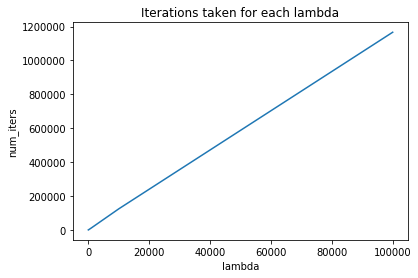
\includegraphics[scale=0.7]{im1}

The result shows that as $\lambda$ increases the number of iterations it takes the algorithm to converge increases (perhaps linearly). This is because when we have large $\lambda$, and starting from $x^{(0)}=[1,2]$, which is an imbalanced start point, (1) the gradient is larger, making the algorithm to take longer time to approach 0 and (2) the learning rate $t$ obtained by backline search is smaller, making the decrease in the gradient even slower every epoch.

\item[d.] 

I ran gradient descent for $[10^0,10^1,10^2,10^3,10^4,10^5]$ (because of run time issue).

Same as c, the result shows that as $\lambda$ increases the number of iterations it takes the algorithm to converge increases (perhaps linearly). The reason is the same as c, but the effect is exacerbated by the fact that the in the update, we're applying the inverse hessian to the update rule as well.

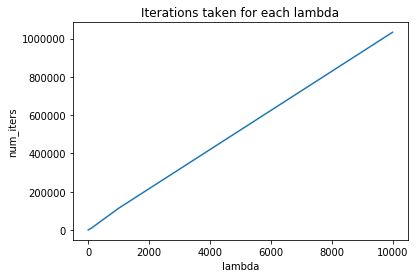
\includegraphics[scale=0.7]{im2}



\end{itemize}
\color{black}



\end{document}
